\begin{frame}
    \frametitle{Discussion}

    \begin{itemize}
        \item Use of dome-shaped flange $\implies$ less skin damage
        \item Electrode cable directly leaving from flange requires simpler surgery \begin{itemize}
            \item Epoxy resin and silicone seal not enough for clinical use. Need hermetic seal.
        \end{itemize}
        \item In TMR, EMG and weight-bearing recovery are coincident \begin{itemize}
            \item Possibly because of surgery, not reinnervation. Suggested a solution how to differentiate.
        \end{itemize}
        \item SNR is not subtle enough, e.g. EMG frequency reduced for reinnervated.
        \item Bipolar electrodes limited to one location
    \end{itemize}

\end{frame}

\begin{frame}
    \frametitle{Conclusion}

    \begin{itemize}
        \item After 19 week recovery, muscle signals recorded reliably
        \item Targeted muscle reinnervation together with bone-anchored prostheses was successful
        \item Support for ITAP as the interface for wires in myoelectric control of prostheses
    \end{itemize}

\end{frame}

\begin{frame}
    \frametitle{Implications}

    \begin{figure}[h]\centering
        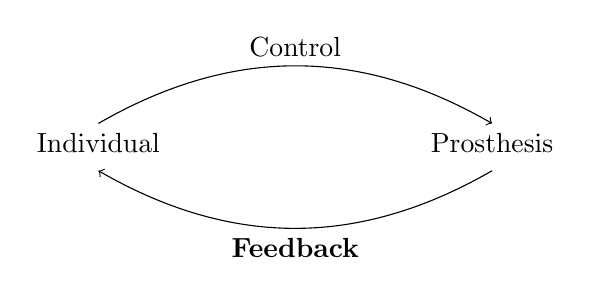
\begin{tikzpicture}
            \draw[->] (0,0) node[below]{Individual} to[bend left] node[midway,above]{Control} (5,0) node[below]{Prosthesis};
            \draw[->] (5,-0.6) to[bend left] node[midway,below] {\textbf{Feedback}} (0,-0.6);
        \end{tikzpicture}
    \end{figure}
    \begin{itemize}
        \item Use of osseoperception \footcite{ClementeFrancesco2017TaHM} \footcite{ÖrgelMarcus2021Oito} \begin{itemize}
            \item Vibrotactile feedback directly onto bone
        \end{itemize}
    \end{itemize}
\end{frame}